\documentclass[12pt]{article}
\title{Mini Report \#2: Sentiment Analysis on Financial News}
\author{Andre Sealy, Daiki Ishiyama, Swapnil Pant}
\usepackage{amsmath, amsfonts, amssymb, amsthm,}
\usepackage{tikz}
\usetikzlibrary{matrix,positioning}
\tikzset{bullet/.style={circle,fill,inner sep=2pt}}
\usepackage{braket}
\usepackage{bbold}
\usepackage[margin=1.0in]{geometry}
\usepackage{mathtools}
\usepackage{xfrac}
\usepackage{xcolor}
\newcommand{\lam}{$\lambda$}
\usepackage{pgfplots}
\tikzset{My Style/.style={samples=100, thick}}
\usepackage{graphicx}
\usepackage{pgfplots}
\usepackage{setspace}
\usepackage{enumerate}
\usepackage{hyperref}
\usepackage{array}
\usepackage{listings}
\usepackage[official]{eurosym}
\usepackage[shortlabels]{enumitem}
\usepackage{booktabs}
\usepackage{floatrow}
\usepackage{listings}
\floatsetup[table]{capposition=top}
\usepackage{appendix}
\usepackage{xcolor}
\hypersetup{
	colorlinks,
	linkcolor={red!50!black},
	citecolor={blue!50!black},
	urlcolor={blue!80!black}
}

\definecolor{codegreen}{rgb}{0,0.6,0}
\definecolor{codegray}{rgb}{0.5,0.5,0.5}
\definecolor{codepurple}{rgb}{0.58,0,0.82}
\definecolor{backcolour}{rgb}{0.95,0.95,0.92}

\lstdefinestyle{mystyle}{
	backgroundcolor=\color{backcolour},   
	commentstyle=\color{codegreen},
	keywordstyle=\color{magenta},
	numberstyle=\tiny\color{codegray},
	stringstyle=\color{codepurple},
	basicstyle=\ttfamily\footnotesize,
	breakatwhitespace=false,         
	breaklines=true,                 
	captionpos=b,                    
	keepspaces=true,                 
	numbers=left,                    
	numbersep=5pt,                  
	showspaces=false,                
	showstringspaces=false,
	showtabs=false,                  
	tabsize=2
}
\onehalfspacing

\lstset{style=mystyle}

\begin{document}
	
\maketitle

\section*{Introduction}

Trend-following strategies -- like moving averages or time-series momentum -- are widely used in practice and have been successful across many different asset classes for decades. Despite their popularity, whether or not investors can generate excess remains questionable. Many existing trend signals are heuristic-based and chosen based on intuition or empirical trial-and-error rather than a grounded, model-based approach. This motivates our question:  Can visual patterns in historical price charts predict whether a stock will rise or fall over the next 5 days?

With the rise of machine learning, there is an opportunity to learn price trends directly from data rather than imposing rigid parametric structures (like fixed-length moving averages). We examine price trends through the lens of supervised learning, treating the trend signal as something that can be trained to predict returns. We aim to bridge the gap between statistical modeling and practical trading signals. We will generate a framework that generalizes popular tend signals and allows for a data-driven optimal trend filter, which improves return predictability and economic outcomes.

\section*{Data \& Preprocessing}
\subsection*{Data Description}

For the project, we use two different datasets that are both structured and unstructured. The structured dataset stock information, while the unstructured involves news articles related to the stock in our analysis.

\subsection*{Stock Prices}

The stock price dataset contains daily stock prices between January 3, 2017, and December 30, 2021. The dataset is relatively simple, as there are only three features: the stock's closing price, the date of the closing price, and the stock's ticker. The dataset contains 480 different equities, including the ticker for the S\&P 500 index, a significant stock price index based in the United States, which lists 500 of the largest multinational companies in the world.

\subsection*{News Articles}

The news articles dataset contains 20,550 news articles, which involves articles published between January 3, 2017, and December 2020. The features include the publication date, the news article headline, the full-text content, and the company mentioned in the article, which we have in the form of a ticker. The news articles cover roughly 381 equities, nearly 100 less than the equities in our stock price dataset. However, the general idea is to analyze how this information can lead to predictions in the equity market.

\begin{figure}[h]
	\centering
	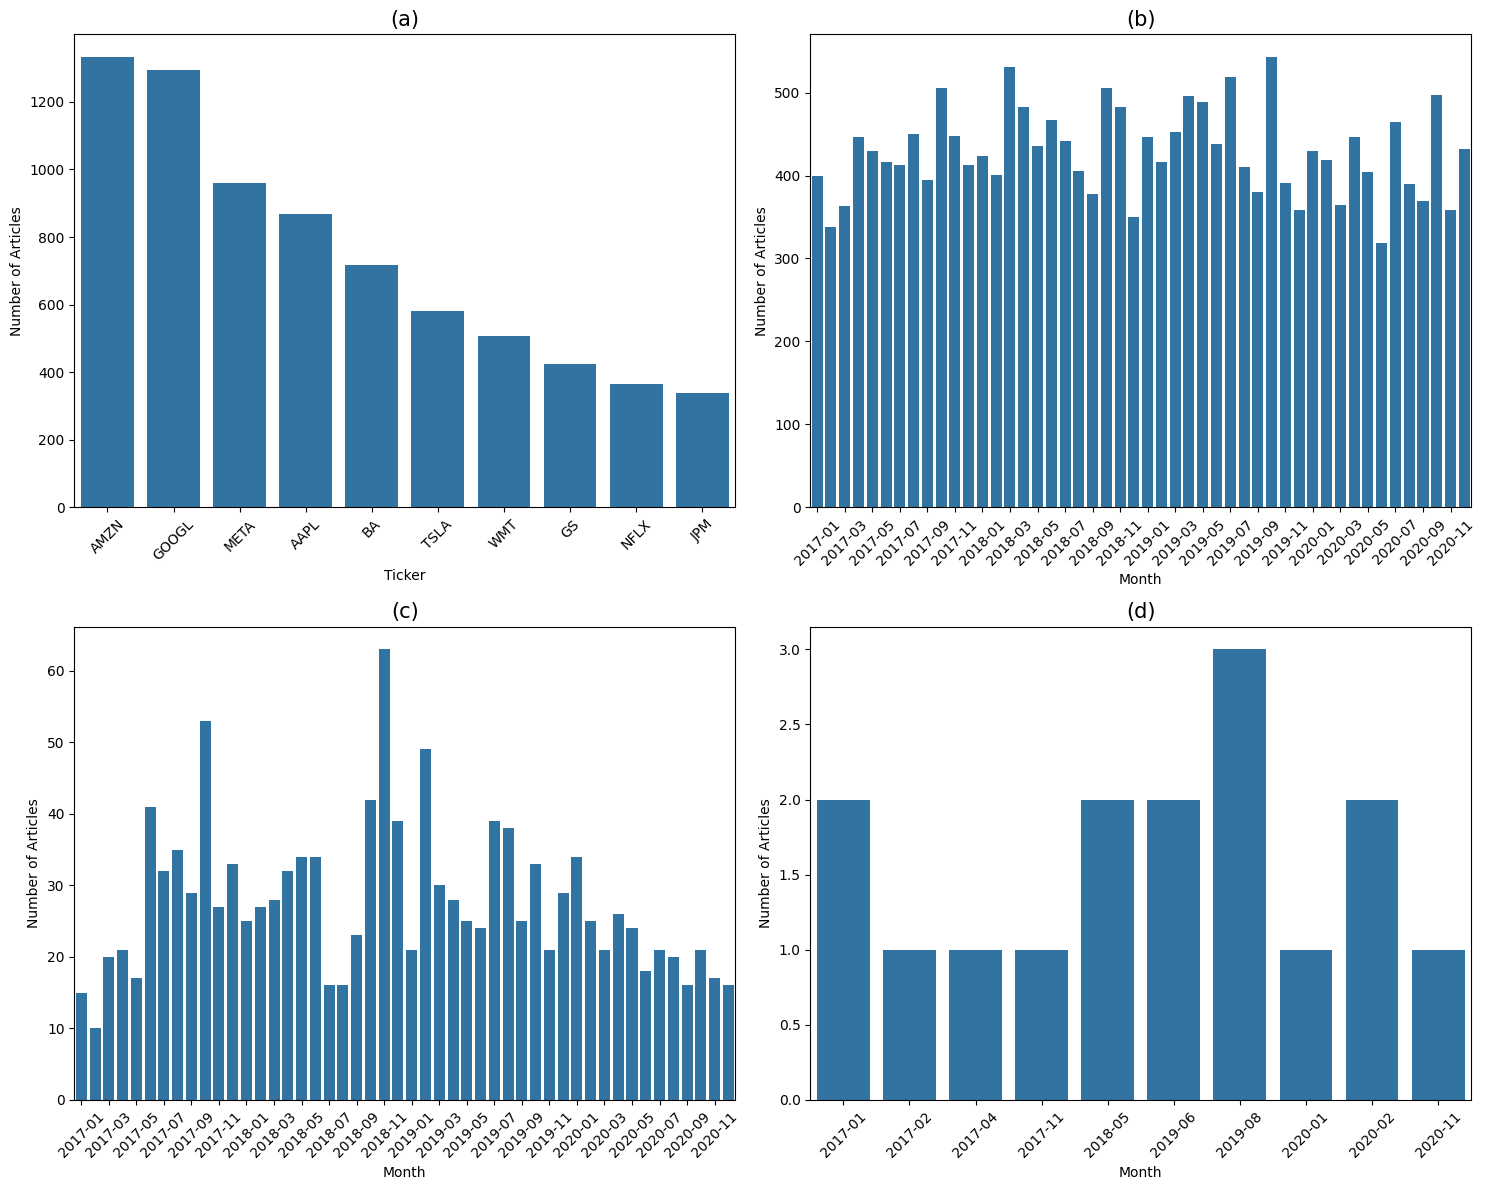
\includegraphics[width=0.9\linewidth]{plots/descriptive.png}
	\caption{Descriptive Plots for News Articles}
	\label{fig:descriptive}
\end{figure}

Figure (\ref{fig:descriptive}) gives us an idea of the different descriptive statistics involved with the amount of articles in our dataset. Plot (a) is a bar chart that shows the top tickers with the highest number of associated news articles in our dataset. As we can see, these companies would include Amazon (AMZN), Google (GOOGL), Meta (META), Apple (AAPL), Boeing (BA), Tesla (TSLA), Walmart (WMT), Goldman Sachs (GS), Netflix (NFLX), and J.P. Morgan Chase \& Co. It should come as no surprise that the largest companies in the world tend to have more articles written about them. JPM and GS are not as large as the other firms in the plot; however, JPM is America's largest universal bank (by deposits and assets), while GS is America's largest pure investment bank.

Plot (b) displays the monthly articles published across the entire dataset, which averages between 350 and 500 articles. In plot (c), we have isolated the news volume specific to AMZN. The distribution reflects significant variability in coverage over time, with spikes that may correspond to product launches, earnings reports, or market-moving announcements. On the other hand, we have the article frequency for YUM Brands (d), where there is sparse coverage, with typically fewer than three articles per month. The lower frequency introduces challenges such as data sparsity and increased noise. This presents challenges when predicting individual stocks based on sentiment.


\section*{Methodology}

This section will outline two methods we have used for our sentiment analysis: the pretrained large language model and the Fine-tuned model. We will also outline the pre-processing required for each of these methods, as they have unique attributes for creation.

\subsection*{Pretrained FinBERT}

Financial markets are increasingly influenced by news and sentiment, making sentiment analysis a crucial tool for market prediction. We explore the application of pretrained FinBERT, a specialized BERT model fine-tuned for financial text analysis, to predict stock market movements based on news sentiment. FinBERT leverages the power of transformer-based language models to capture nuanced financial sentiment, offering a sophisticated approach to market analysis.

\subsubsection*{Model Architecture}

FinBERT is built upon BERT architecture, which is short for Bidirectional Encoder Representation from Transformer. There are many different FinBERT architectures one can utilize. However, we are using the architecture developed by Yi Yang, Allen Huang, and Hui Wang (yiyanghkust) at the Hong Kong University of Science and Technology. The base architecture has 12 transformer layers, a hidden size of 768 dimensions, and 12 attention heads, which gives us a total of ~110 million parameters.

The yiyanghkust model comes with an embedding layer, transformer encoder, pooling layer, and classification header, along with domain-specific applications for reading financial documents. At its core, this layer combines three distinct embedding types: word embedding (with a vocabulary of 30,522 tokens), positional embeddings (which capture sequence order up to 512 tokens), and token type embeddings (which help distinguish token pairs). Each embedding operates in a 768-dimensional space, comprehensively representing financial text. This layer structures the specialized financial vocabulary, including market-specified terminology, company names, and financial jargon, all pretrained on financial documents.

The pooling layer transforms sequence-level representations into a fixed-dimensional vector for classification task. This layer specifically processes the classification token [CLS] representation, which aggregates information from the entire input sequence through the transformer layers. The pooling mechanism involves a linear transformation that maps the 768-dimensional hidden state to another 768-dimensional space, which is then followed by a Tanh activation function. This non-linear transformation helps capture complex patterns in the financial text while maintaining the model's ability to represent both positive and negative sentiment.

The classification head in FinBERT transforms the pooled representation into sentiment predictions through a linear layer that maps the 768-dimensional input to three output neurons, which corresponds to positive, neutral, and negative sentiment classes. This layer applies a softmax activation function to convert the raw logits into probability distributions, enabling the model to quantify the confidence of its sentiment predictions.

\subsubsection*{VADER Sentiment}

We've also implemented VADER (Valence Aware Dictionary and sEntiment Reasoner), a rule-based sentiment analysis tool specifically designed for social media text. It uses a pre-built lexicon of sentiment-related words, each scored for their positive and negative intensity, along with rules for handling modifiers, capitalization, and punctuation. Like the FinBERT pretrained model, the VADER model produces positive, negative, and neutral sentiment, but it also produces the fourth score, which is a compound normalization score between -1 and 1. While less sophisticated than FinBERT, VADER provides a computationally efficient baseline for sentiment analysis and is particularly effective at capturing sentiment in shorter text, such as article headlines. Using this metric, we can assess if the headline captures a different sentiment than what is conveyed in the body of the article. Media experts and analysts would consider this inconsistency "engagement bait."

\subsubsection*{Sentiment Preprocessing}

The pretrained sentiment pipeline implements a dual-model approach combining FinBERT and VADER to analyze financial news sentiments. The FinBERT analysis utilizes the yiyanghkust, which is trained explicitly for financial text analysis. This function first tokenizes input text using a maximum sequence length of 512 tokens, handling longer texts through truncation. The model then processes the tokenized input through its transformer architecture, producing logits converted to probabilities via softmax activation. The resulting sentiment is mapped to a continuous scale from -1 (strongly negative) to 1 (strongly positive), with 0 representing a neutral sentiment.

Parallel to this, the VADER sentiment analysis provides a rule-based alternative. VADER analyzes the text using its specialized lexicon and scoring rules, producing separate positive, negative, and neutral sentiment scores. The function selects the dominant sentiment and maps it to the same -1 to 1 scale as FinBERT, ensuring compatibility between the two approaches. After processing all articles, the system combines the results from FinBERT and VADER by averaging both scores into a combined sentiment score. The combined approach leverages the strengths of FinBERT's sophisticated understanding of financial context and VADER's efficient processing of shorter text.

\subsection*{Fine-Tuned BERT}

Here, we are adapting a pretrained BERT model for the specific downstream tasks. Fine-tuning a BERT model involves taking a pre-trained transformer-based language model, such as BERT (Bidirectional Encoder Representations from Transformers), which has already learned contextualized representations from large-scale text data, and further training it on a task-specific dataset. During fine-tuning, the model updates its weights slightly, adapting its deep contextual understanding of language to a specific downstream task like sentiment analysis, text classification, or named entity recognition. This approach significantly reduces training time and computational resources compared to training from scratch, leveraging BERT's ability to capture linguistic nuances.

Utilizing a fully connected neural network (FCNN) as a classifier on top of a fine-tuned BERT model allows for effective interpretation of the learned features from BERT's embedding layers. After obtaining contextual embeddings from BERT, these embeddings are passed through the FCNN, typically consisting of one or more hidden layers with nonlinear activation functions, to perform task-specific classification or regression. The fully connected layers help the model capture nonlinear relationships and perform complex transformations, enhancing its ability to generalize and improving prediction accuracy on targeted tasks.

\subsubsection*{Data Preprocessing}

The stock price data undergoes initial transformation to calculate daily returns, which are computed using percentage changes in closing prices grouped by ticker symbols. This step establishes the foundation for measuring price movements that will later serve as the basis for sentiment labels. Missing values are removed to ensure data quality, and date fields are standardized to enable proper temporal alignment of news and price data. Binary labels are generated based on the direction of price movements, where positive returns are encoded as 1 and negative returns as 0. These labels are converted to float type to ensure compatibility with the model's loss function and training process.

We use a temporal split strategy, dividing the dataset into training, validation, and test sets. Data before 2019 is allocated for training, 2019 data for validation, and 2020 onwards for testing. This chronological splitting is crucial for maintaining the temporal nature of financial data and ensuring that the model's evaluation reflects its ability to generalize to future, unseen data. This approach prevents look-ahead bias and objectively assesses the model's performance.

We also implement HuggingFace's dataset infrastructure, a sophisticated processing framework designed explicitly for transformer-based models using specialized dataset objects. The Dataset framework organizes our financial data into a columnar format, maintaining distinct features, including the processed text (combined news titles and bodies), binary sentiment labels derived from price movements, and subsequently generated attention masks and input IDs. This structure facilitates efficient access patterns and rapid data retrieval during training. The framework preserves the chronological nature of our data split across training (pre-2019), validation (2019), and testing (2020 onwards) sets, ensuring temporal consistency in our financial sentiment analysis.

Afterward, we initialize the BERT tokenizer, explicitly using the 'bert-base-uncased' model. This tokenizer is fundamental to our approach as it implements WordPiece tokenization, a sophisticated method that breaks down text into subword units. The uncased version is chosen to standardize all text to lowercase, reducing vocabulary complexity while maintaining semantic meaning. Then, we apply the tokenization process across the training, validation, and testing datasets. This transformation adds new features to our dataset, which involves the input IDs that represent the numerical encoding of our text and attention masking that differentiates between actual tokens and padding.


\subsubsection*{Model Architecture}

The architecture combines a pretrained BERT model with a custom classification head to perform financial sentiment analysis. It begins with the bert-base-uncased foundation model, whose parameters are initially frozen. Freezing BERT’s weights at the start helps preserve its general language understanding while allowing the newly added classifier layers to learn the specific nuances of financial sentiment.

On top of the frozen BERT outputs (768-dimensional embeddings), the classifier features a progressively smaller feed-forward network that reduces dimensions through three main stages:

\[
	768\rightarrow 512\rightarrow 256\rightarrow 128\rightarrow 1
\]

At each stage, the architecture applies:

\begin{itemize}
	\item \textbf{Batch Normalization} – to stabilize training by normalizing layer inputs.
	\item \textbf{ReLU Activation} – to introduce nonlinearity and improve modeling capacity.
	\item \textbf{Dropout} – to combat overfitting by randomly “dropping” neurons (with rates of 0.3 and 0.2)
\end{itemize}

This systematic reduction and regularization strategy helps distill the essential sentiment information from BERT’s rich language representations.

During the forward pass, tokenized text is fed into the frozen BERT layers to generate contextual embeddings. These embeddings are then passed through the classifier layers to produce sentiment predictions. When labels are provided, Binary Cross Entropy with Logits Loss is used to train the network for binary (positive/negative) sentiment classification. Overall, this design strikes a balance between leveraging BERT’s robust language modeling capabilities and tailoring the model specifically for financial sentiment tasks.

\subsubsection*{Hyperparameter Variations}

\begin{table}[ht]
	\centering
	\begin{tabular}{@{} l l l l l l @{}}
		\toprule
		\textbf{} & \textbf{Model} & \textbf{Classifier Dimensions} & \textbf{Dropout} & \textbf{Activation} & \textbf{Normalization} \\
		\midrule
		A & bert-base-uncased & 768 $\rightarrow$ 512 $\rightarrow$ 256 $\rightarrow$ 128 $\rightarrow$ 1 & 0.3, 0.3, 0.2 & ReLU & BatchNorm1d \\
		B & finbert-tone      & 768 $\rightarrow$ 512 $\rightarrow$ 256 $\rightarrow$ 128 $\rightarrow$ 1 & 0.3, 0.3, 0.2 & ReLU & BatchNorm1d \\
		C & finbert-tone      & 768 $\rightarrow$ 384 $\rightarrow$ 192 $\rightarrow$ 1                    & 0.5, 0.4, 0.3 & ReLU & LayerNorm \\
		D & bert-large-uncased & 768 $\rightarrow$ 1024 $\rightarrow$ 512 $\rightarrow$ 256 $\rightarrow$ 1 & 0.3, 0.3, 0.2 & GELU & BatchNorm1d \\
		\bottomrule
	\end{tabular}
	\caption{Overview of Four Different Experimental Setups}
	\label{tab:experiments}
\end{table}

Table (\ref{tab:experiments}) shows an illustration of four different experiment setups. Our experiments examined multiple hyperparameter variations across dropout rates, classifier dimensions, normalization layers, activation functions, and model backbones. In addition to the bert-base-uncased model, we have also experimented with bert-large-uncased and pretrained models such as the yiyanghkust.

The feed-forward layers for experiments A and B systematically compress these high-dimensional embeddings into a final scalar for binary classification. Reducing the dimensionality step by step helps filter out unnecessary information and focus on the most relative features for the sentiment task. In experiment C, the network compresses more aggressively, as this reduction trims the feature space more quickly and can help lower the risk of overfitting (at the risk of limiting the model's capacity to learn more nuanced patterns). Experiment D expands the first layer to 1024 before stepping back down. This larger "widening" may be better for capturing more complex patterns, which comes at the cost of increased computation.

In terms of the activation functions, experiments A and B utilize a simple ReLU function, which zeros out negative inputs and keeps positive values. ReLU pairs well with batch normalization, stabilizing the distribution of intermediate activation and improving training convergence. On the other hand, the experiment utilizes layer normalization, which normalizes token representation across feature dimensions. This can be beneficial for smaller or more variable batch sizes. Experiment D utilizes the Gaussian Error Linear Unit (GELU), which has a smoother function than ReLU, blending elements of sigmoid-like gating and linear transformations.

\section*{Model Evaluation}

The following section outlines the analyze the performance between the pretrained and fine-tuned models. We cover the metrics used to assess the performance of both models, as well as unique attributes we've applied to the testing criteria that improves performance. To assess the efficacy of our pretrained BERT, we have decided to integrate elements of a Long Short-Term Memory model architecture, or LSTM. LSTM networks are a specialized type of Recurrent Neural Network (RNN) designed to overcome the limitations of traditional RNNs in handling long-term dependencies. They are particularly effective for sequential data analysis and ideal for time series prediction.

To compare the performance of our integrated BERT-LSTM model, we have run a performance evaluation using a simple Multilayer Preceptron (MLP) model as a baseline, as well as a standard LSTM model. 


\subsubsection*{Multilayer Perceptron}

The Multilayer Perceptron (MLP) is a simple, fully connected Feed-Forward Artificial Neural Network (ANN). It has three hidden layers between the input and output layers. The first, second, and third layers use 50, 30, and 20 units, respectively, each with a Tanh activation function afterward. After each layer, we utilize a dropout layer: 0.15 for the first layer, 0.05 for the second layer, and 0.01 for the third. Finally, the output layer uses a linear activation function similar to the FinBERT-LSTM. These weights and biases are adjusted during backpropagation, where optimizers such as Adam are used to minimize the Mean Squared Error, which we use for our loss function.

\subsubsection*{Long Short-Term Memory}

Long Short-Term Memory (LSTM) allows a model to remember previous information for more extended periods. An LSTM cell consists of 3 gates: the Input, Output, and Forget gates. The input gate controls the flow of input activations into the memory cell, given by 

\begin{equation}
	i_i=\sigma(W_i\times\left[h_{t-1}, X_t\right]+b_i)
\end{equation}
where $i_t$ is the output of the input gate at time step $t$, $W_i$ is the weight of the input gate, $h_{t-1}$ is the hidden state at time step $t-1$, and $X_t$ is the input at time step $t$ and $b_i$ is the bias of the input gate. We also have to consider the candidate value given by the following

\begin{equation}
	\hat{c}=\tanh(W_c\times\left[h_{t-1},X_t\right]+b_c).
\end{equation}
The candidate value is added to the output at time step $t$, $W_c$ is the weight of the candidate value, and $b_c$ is the bias of the candidate value. The forget cell controls which information to remember and which to forget in memory. It is given by

\begin{equation}
	f_t=\sigma(W_f\times\left[h_{h-1},X_t\right]+b_f)
\end{equation}
where $f_t$ is the output of the forget gate at time step $t$, $W_f$ is the weight of forget gate, and $b_f$ is the bias of the forget gate. The output gate controls the information taken from the output memory cell, given by

\begin{equation}
	o_t=\sigma(W_o\times\left[h_{t-1},X_t\right]+b_o)
\end{equation}
where $o_t$ is the output of the output gate at time step $t$, $W_o$ is the weight of the output gate, $b_o$ is the bias of the output gate. We also have the new cell state
\begin{equation}
	c_t=f_t\times c_{t-1}+i_t\times\hat{c}_t
\end{equation}
where $c_t$ is the new cell state at time step $t$. The hidden state at time step $t$ is given by
\begin{equation}
	h_t=o_t\times\tanh(c_t)
\end{equation}

\subsubsection*{BERT-LSTM}

The FinBERT integration and LSTM allow us to use textual information from news for short-term stock movements. The FinBERT-LSTM model takes the sequence length, as well as the sentiment score, which is provided from the sentiment preprocessing step. The overall architecture uses three layers in total. The first layer has 70 memory units (hidden states) as well as a Tanh activation function for the cell state. Since the output of the Tanh function is -1 to 1, the bounded range helps prevent exploding gradients during backpropagation, as well as numerical instability in long sequences. The first layer is also used to capture many temporal patterns. Also, a large number of units allows the layer to learn complex patterns.

The second LSTM layer uses the same activation function but with fewer memory cells (30). This reduces the dimensionality while maintaining temporal information, which helps learn abstract features. The third and final layer produces a single vector from a memory cell of 10 units. This memory cell acts as a bottleneck layer, used only for the final output. The output layer will use the linear activation function.

\subsubsection*{Evaluation Metrics}
We utilize 5 different evaluation metrics, the first of which is $R^2$. In addition to computing the $r^2$, we calculate the Mean Absolute Error (MAE). The Mean Absolute Error is the mean of the distance between the target variable and predicted value, computed by 
\begin{equation}
	\text{MAE}=\frac{\sum_{i=1}^{n}|\hat{y}_i-y_i|}{n}
\end{equation}
where $\hat{y}_i$ is the predicted value for training example $i,y_i$ is the target variable for training example $i$. We also compute the Mean Absolute Percentage Error (MAPE), the mean of the distance between the target variable and the predicted value as a fraction of the target variable. MAPE can be computer by
\begin{equation}
	\text{MAPE}=\frac{1}{n}\sum_{i=1}^{n}\left|\frac{\hat{y}_i-y_i}{y_i}\right|.
\end{equation}
We also compute the accuracy, which is the inverse of the MAPE,
\begin{equation}
	\text{Accuracy}=1-\text{MAPE}.
\end{equation}
Using the predicted binary classifications, along with the actual binary classifications, allows us to compute the F1-Score, which is derived from the following
\begin{equation}
	\text{F1-Score}=2\cdot\frac{\text{Precision}\times\text{Recall}}{\text{Precision}+\text{Recall}}
\end{equation}
where the Precision and Recall are derived by the following
\begin{equation}\label{eq:f1score}
	\text{Precision}=\frac{\text{TP}}{\text{TP}+\text{TN}}\quad\text{Recall}=\frac{\text{TP}}{\text{TP}+\text{TN}}.
\end{equation}
As always TP represents the True Positives, FP are the False Positives and the FN are False Negatives.

\subsubsection*{Pre-trained Performance}

As mentioned previously, to compare the training performance of the MLP, LSTM, and FinBERT-LSTM models, we implement three hidden layers. All models utilize the same number of units in each layer, as well as the same activation function for each layer and dropout rate. We normalize our data using min-max normalization, as well as an MSE loss function and Adam optimizer with a learning rate of 0.01. Each model will also utilize a sequence length of 10, with 15 epochs for training and validating.

\begin{table}[ht]
	\centering
	\begin{tabular}{@{} l c c c c c @{}}
		\toprule
		\textbf{Model} & \textbf{MAE} & \textbf{MAPE} & \textbf{Accuracy} & $R^2$ & \textbf{F1-Score} \\
		\midrule
		MLP & 14.1440  & 0.1119 & 0.8880 & 0.9605 & 0.5241 \\
		LSTM & 16.1575  & 0.1112 & 0.8887 & 0.9248 & 0.5218 \\
		FinBERT-LSTM  &  37.7389 & 0.0085 & 0.9914 & 0.9998 & 0.5853  \\
		\bottomrule
	\end{tabular}
	\caption{Overview of Four Different Experimental Setups}
	\label{tab:pretrained}
\end{table}

Table (\ref{tab:pretrained}) shows the performance between the MLP, LSTM, and FinBERT-LSTM models. As we can see, the LSTM performs better than the baseline MLP and LSTM. Considering the well-conditioned FinBERT embeddings, the layers with the $\tanh$ activation function allow for fewer extremes. Also, since FinBERT was already fine-tuned on tasks such as sentiment classification and next-sentence prediction in news articles, FinBERT is good at handling what is said, while LSTM handles when things matter.

\subsection*{Fine-Tuned BERT}

\begin{table}[h!]
	\centering
	\caption{Hyperparameter Configurations for BERT Experiments}
	\begin{tabular}{lcccl}
		\hline
		 \textbf{Model Architecture} & \textbf{Learning Rate} & \textbf{Batch Size} & \textbf{Epochs} & \textbf{Activations} \\ \hline
		BERT-base & $2\times 10^{-5}$ & 32 & 15 & ReLU, Linear \\[3pt]
		 (768 $\rightarrow$ 512$\rightarrow$ 256 $\rightarrow$ 128 $\rightarrow$ 1) & & &&  \\ 
		FinBERT-tone & $3\times 10^{-5}$ & 16 & 15 & ReLU, Linear \\[3pt]
		 (768 $\rightarrow$ 512$\rightarrow$ 256 $\rightarrow$ 128 $\rightarrow$ 1) & & &&  \\ 
		FinBERT-tone & $2\times 10^{-5}$ & 32 & 15 & ReLU, Linear \\[3pt]
		 (768 $\rightarrow$ 384 $\rightarrow$ 192 $\rightarrow$ 1) & & &  &\\ 
		BERT-Large-uncase & $1\times 10^{-5}$ & 8 & 15 & GELU, Linear \\[3pt]
		 (1024 $\rightarrow$ 1024 $\rightarrow$ 512 $\rightarrow$ 256$\rightarrow$1) & & &&\\ \hline
	\end{tabular}
	\label{tab:hyperparams}
\end{table}

Considering that the fine-tuned experiments are more sophisticated that what was previously outlined, we take the time outline more details about the model architecture for our experiment. All of the models ran for 15 epoch for both the training and validation set. However, we use a slightly higher learning rate for the BERT-base architecture. This is because the $\tanh$ activation function tends to shrink the gradient magnitudes compared to the ReLU or GELU. 

Model D uses the smallest learning rate with the smallest batch size, allowing us to regularize models with many parameters (BERT-Large-uncased has ~340 million parameters). This will also be helpful, since we can keep our step sizes very small. Instead of using the ReLU for our activation functions, we have opted to go with the GELU since the small learning rates allow us to have more precise steps.

Table (\ref{tab:performance_metrics}) shows the performance metrics of different fine-tuned BERT models, where we compare the accuracy, MSE, $R^2$ and F1-Score. Since the data is very noisy, not continuous or linearly predictable, we would not expect to have a positive, or meaningful $R^2$. However, the other metrics are still very useful.

As we can see, model experiment D shows the highest accuracy rate of 0.5178, which means that the model is able to accurately predict the sentiment of financial news articles 51.58\% of the time. This may be due to the deeper, fully connected neural network, which allows the model to capture more nonlinearities. This model also has a lower learning rate (1e-5) and smaller batch size (8), which allows more granular updates, reducing overfitting and helping it generalize slightly better.

\begin{table}[h!]
	\centering
	\caption{Performance Metrics Comparison of BERT Experiments}
	\begin{tabular}{ccccc}
		\hline
		\textbf{Experiment} & \textbf{Accuracy (\%)} & \textbf{MSE} & $R^2$ & \textbf{F1-Score} \\ \hline
		A & 51.12 & 0.2512 & -0.0049 & 0.5909 \\ 
		B & 49.67 & 0.2516 & -0.0068 & 0.5971 \\ 
		C & 49.35 & 0.2504 & -0.0016 & \color{red}\textbf{0.6606} \\ 
		D & \color{red}\textbf{51.78} & 0.2507 & -0.0028 & 0.5159 \\ \hline
	\end{tabular}
	\label{tab:performance_metrics}
\end{table}

On the other hand, the accuracy metric can be misleading due to imbalanced datasets. However, the outcome from our test predictions shows that the pre-trained model has analyzed 2,414 positive articles and 2,478 negative articles. Still, we look to the F1-score, the derivation of which can be seen in equation (\ref{eq:f1score}). As we can see, model C achieves the highest F1-score of 0.6606. We do not consider model C to be particularly unique, so there may be some reasons behind this score.

One reason for the high F1-Score may be the moderate depth of the architecture, enough to learn nonlinear decision boundaries but not so deep to overfit (this is supported by achieving a relatively high $R^2$). This allows us to avoid the extremes of too shallow or too wide models from experiments A and D. Another reason is that model C uses the FinBERT-tone architecture, developed by yiyanghkust, which has already been shown to be a fairly concise and accurate model. Overall, we know that the F1-score allows us to minimize false positives and negatives, especially in hard-to-classify examples. We find that the model that performs the best is the model that balances accuracy and the F1-score, which is model D.

\begin{figure}[h]
	\centering
	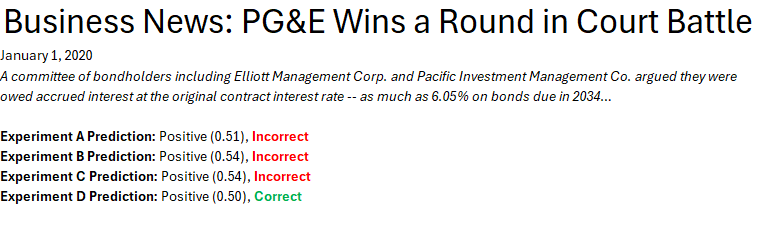
\includegraphics[width=1\linewidth]{plots/outcome.png}
	\caption{Predictive Sentiment for a Sample News Article}
	\label{fig:outcome}
\end{figure}

Figure (\ref{fig:outcome}) shows a sample prediction for one of the articles in our test set. The article's subject involves a legal battle with Pacific Gas and Electric Company (PCG). The article initially appeared in the Wall Street Journal on January 1st, 2020 (the original article can be found \href{https://www.wsj.com/articles/pg-e-bankruptcy-court-rules-against-bondholders-in-interest-rate-fight-11577829961}{here}). Upon reading the article, it appears there are issues related issues on PCG's ability to pay accrued interests on its debt. From the article, a casual reader would suggest that the overall tone and sentiment of the topic are negative. Were the models able to predict the sentiment? As it turned out, the pre-trained FinBERT was able to assess that the overall sentiment of this article is negative (FinBERT score: -0.999073, VADER score: 0.488, Combined score: -0.255537). However, only model D was able to accurately predict the sentiment of the model.

\section*{Sentiment and Market Trend}

\begin{figure}[h]
	\centering
	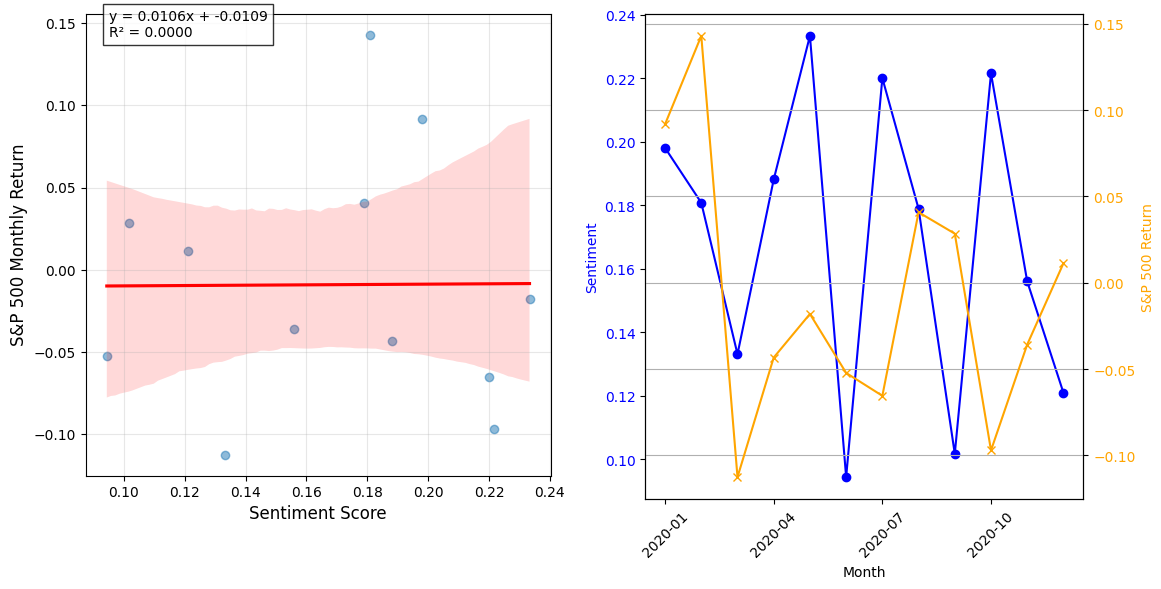
\includegraphics[width=1\linewidth]{plots/regression_time_pretrain.png}
	\caption{Regression and Time Series Plot for the Pre-Trained FinBERT Model}
	\label{fig:pretrain_time_regression}
\end{figure}


\begin{figure}[h]
	\centering
	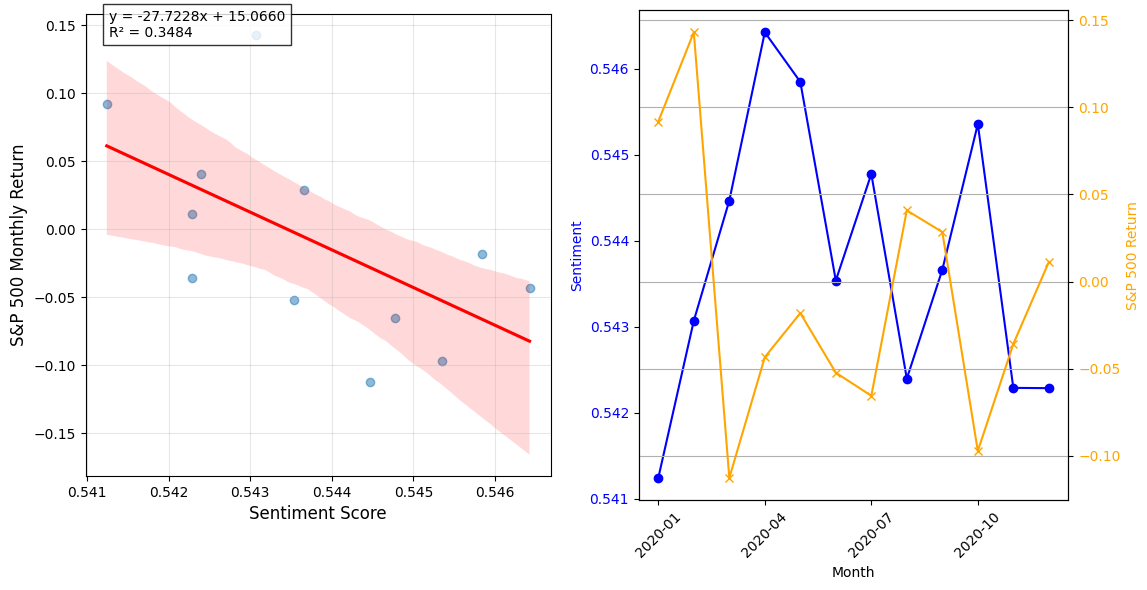
\includegraphics[width=1\linewidth]{plots/regression_time_finetune.png}
	\caption{Regression and Time Series Plot for the Fine-Tuned FinBERT Model}
	\label{fig:finetune_time_regression}
\end{figure}


\section*{Conclusion}



\end{document}